\begin{frame}
  \frametitle{X.509 PKI: hierarchy}
  \vskip -1cm
  \begin{block}{}
    \begin{figure}
      \centering
      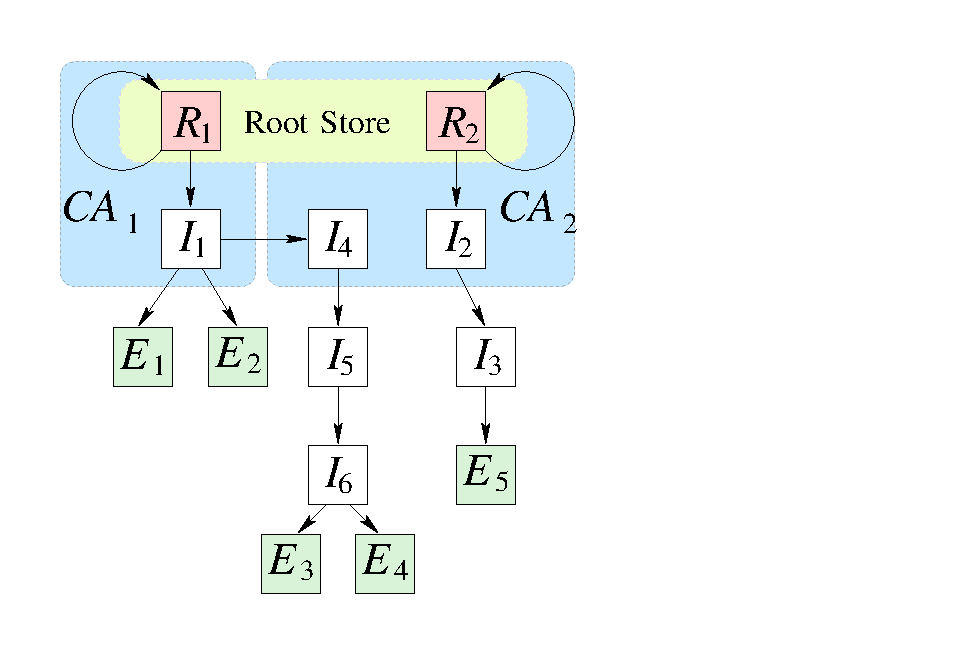
\includegraphics[scale=.7]{figures/x509tree-simplified.pdf}
    \end{figure}
  \end{block}
  \vskip -.7cm
  \begin{block}{\centering All CAs equal. Break one CA, break everything.}\end{block}
\end{frame}




%\begin{frame}
%  \frametitle{One Root Store to Bind Them All}
%  \vskip .1cm
%    \begin{figure}
%    \centering
%     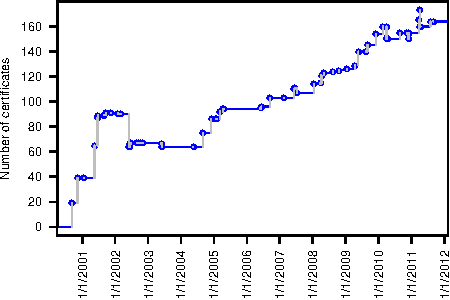
\includegraphics[scale=.9]{plots/cas-in-nss.pdf}
%     \caption{CAs in Mozilla Firefox root store.}
%    \end{figure}
%  \begin{block}{Break one CA, break everything.}\end{block}
%\end{frame}





%\begin{frame}
%  \frametitle{Much activity in recent years}
%  \begin{block}{PKI weaknesses since 2008}
%    \begin{itemize}
%      \item December 2008: Comodo, StartSSL hacks
%      \item March 2011: Comodo CA hacked
%	\begin{itemize}
%	 \item Browsers blacklist $\approx$ 10 certificates
%	\end{itemize}
%      \item July 2011: DigiNotar CA hacked
%	\begin{itemize}
%	  \item 531 rogue certificates \textit{in the wild}
%	\end{itemize}
%    \end{itemize}
%  \end{block}
%\end{frame}


\begin{frame}[fragile]
  \frametitle{Case study: DigiNotar vs. Iran?}
\vskip -.8cm
    \begin{figure}
    \centering
     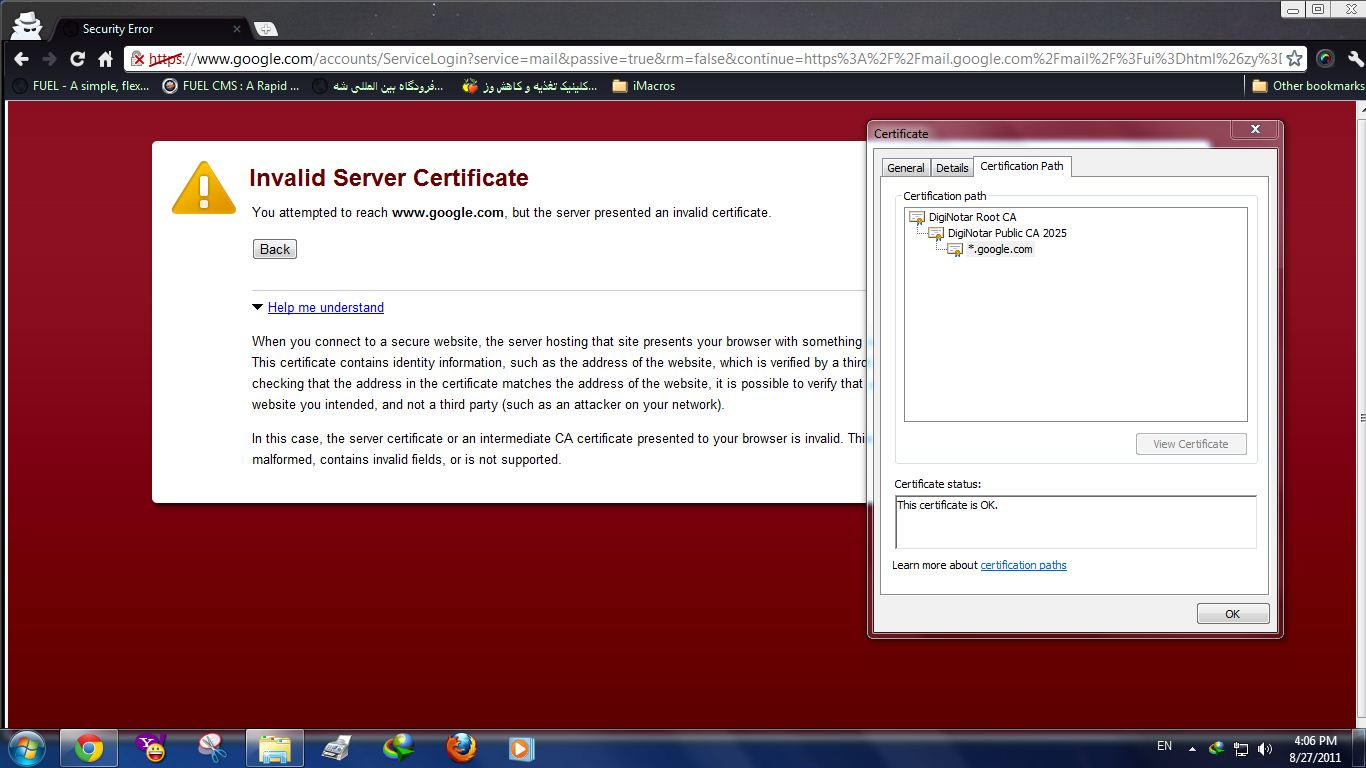
\includegraphics[scale=.37]{figures/gmail_iran.jpg}
    \end{figure}
\end{frame}




\begin{frame}
\frametitle{Crossbear: hunting the MitM}
\begin{block}{This is \textit{not} a proposal to strengthen X.509.}\end{block}
\begin{block}{Crossbear: a tool to gather \textit{hard data}.}
  \begin{itemize}
    \item Raise reliable data about MitM \textit{in the wild}
    \item \textit{How often} do MitM occur?
    \item \textit{Where} are the attackers located?
    \item \textit{Who} are the attackers?
    \item Are we jumping at shadows?
  \end{itemize}
\end{block}
\begin{block}{Method: combine notary principle, tracing and centralised reporting and analysis.}\end{block}
\end{frame}
